\documentclass[11pt]{article}

\usepackage[margin=1in]{geometry}
\usepackage{setspace}
\onehalfspacing
\usepackage{graphicx}
\graphicspath{report_images/}
\usepackage{appendix}
\usepackage{listings}
\usepackage{float}
\usepackage{multirow}
\usepackage{amsthm}
% The next three lines make the table and figure numbers also include section number
\usepackage{chngcntr}
\counterwithin{table}{section}
\counterwithin{figure}{section}
% Needed to make titling page without a page number
\usepackage{titling}

% DOCUMENT INFORMATION =================================================
\font\titleFont=cmr12 at 11pt
\title {{\titleFont ECEN 424: Advanced Digital Design\\ North Carolina Agricultural and Technical State University \\ Department of Electrical and Computer Engineering}} % Declare Title
\author{\titleFont Prepared by: Chris Cannon} % Declare authors
\date{\titleFont 2018-10-10}
% ======================================================================

\begin{document}

\begin{titlingpage}
\maketitle
\begin{center}
	Project 1 Report 
\end{center}
\end{titlingpage}

\section{System Overview}
This system will be a VHDL-based digital lock that must be implemented on the Digilent Basys3 FPGA. The lock will take a 6-digit code, entered via a standard USB numeric keyboard. The code must be re-programmable. The system must notify a user of an incorrect password and must lock permanently after 3 incorrect attempts.

\section{Modules}

\subsection{Module Overview}

The system should include the following modules

\begin{table}[H]
\begin{tabular}{| p{5cm} | p{10.5cm} |}
	\hline
	Module & Description \\ \hline
	main & Main finite state machine and top-level module. \\ \hline
	code\textunderscore timeout\textunderscore timer & Counts to 20 seconds, after which it will notify the main so that the code can be cleared. \\ \hline
	set\textunderscore timeout\textunderscore timer & Counts to 10 seconds, after which it will notify the main so that the set state can be exited \\ \hline
	open\textunderscore timeout\textunderscore timer & Counts to 15 seconds, after which it will notify the main to lock the system \\ \hline
	display\textunderscore timeout\textunderscore timer & Counts to 5 seconds, after which it will notify the display-controller so that the display will be cleared \\ \hline
	clock\textunderscore divider & Divides the clock signal to 4 Hz for the input module to prevent accidental double keystrokes \\ \hline
	input\textunderscore controller & Interprets the keystrokes from the USB keyboard and passes the appropriate command to the main\\ \hline
	output\textunderscore controller & Interprets the command from main and displays the appropriate message on the 7-segment display and LED \\ \hline
\end{tabular}
\end{table}

\subsection{main}

\subsection{Overview}

The main module is the finite state machine that is the top-level component of the system.

\subsubsection{Inputs}

\begin{table}[H]
\begin{tabular}{| p{2.5cm} | p{6cm} | p{6cm} |}
	\hline
	Input Name & Data Type & Description \\ \hline
	cmd & std\textunderscore logic\textunderscore vector(3 downto 0) & Input command from the input\textunderscore controller module. \\ \hline
	code\textunderscore timeout & std\textunderscore logic & Indicates when the code entry has timed out. \\ \hline
	set\textunderscore timeout & std\textunderscore logic & Indicates when the set function has timed out. \\ \hline
	open\textunderscore timeout & std\textunderscore logic & Indicates when the lock should close. \\ \hline
	clk & std\textunderscore logic & Board clock signal \\ \hline
\end{tabular}
\end{table}

\subsubsection{Outputs}

\begin{table}[H]
\begin{tabular}{| p{2.5cm} | p{6cm} | p{6cm} |}
	\hline
	Output Name & Data Type & Description \\ \hline
	enable\textunderscore code & std\textunderscore logic & Activates the code\textunderscore timeout\textunderscore timer module. \\ \hline
	reset\textunderscore code & std\textunderscore logic & Restarts the code\textunderscore timeout\textunderscore timer module. \\ \hline
	enable\textunderscore set & std\textunderscore logic & Activates the set\textunderscore timeout\textunderscore timer module. \\ \hline
	reset\textunderscore set & std\textunderscore logic & Restarts the set\textunderscore timeout\textunderscore timer module. \\ \hline
	enable\textunderscore open & std\textunderscore logic & Activates the open\textunderscore timeout\textunderscore timer module. \\ \hline
	reset\textunderscore open & std\textunderscore logic & Restarts the open\textunderscore timeout\textunderscore timer module. \\ \hline
	display\textunderscore cmd & std\textunderscore logic\textunderscore vector(3 downto 0) & Binary encoded message for the output\textunderscore controller module. \\ \hline
\end{tabular}
\end{table}

\subsection{code\textunderscore timeout\textunderscore timer}

\subsubsection{Inputs}

\begin{table}[H]
\begin{tabular}{| p{2.5cm} | p{6cm} | p{6cm} |}
	\hline
	Input Name & Data Type & Description \\ \hline
	enable & std\textunderscore logic & Activates the code\textunderscore timeout\textunderscore timer module. \\ \hline
	reset & std\textunderscore logic & Restarts the code\textunderscore timeout\textunderscore timer module. \\ \hline
	clk & std\textunderscore logic & Board clock signal \\ \hline
\end{tabular}
\end{table}

\subsubsection{Outputs}

\begin{table}[H]
\begin{tabular}{| p{2.5cm} | p{6cm} | p{6cm} |}
	\hline
	Output Name & Data Type & Description \\ \hline
	done & std\textunderscore logic & Indicates when the code entry has timed out. \\ \hline
\end{tabular}
\end{table}

\subsection{set\textunderscore timeout\textunderscore timer}

\subsubsection{Inputs}

\begin{table}[H]
\begin{tabular}{| p{2.5cm} | p{6cm} | p{6cm} |}
	\hline
	Input Name & Data Type & Description \\ \hline
	enable & std\textunderscore logic & Activates the set\textunderscore timeout\textunderscore timer module. \\ \hline
	reset & std\textunderscore logic & Restarts the set\textunderscore timeout\textunderscore timer module. \\ \hline
	clk & std\textunderscore logic & Board clock signal \\ \hline
\end{tabular}
\end{table}

\subsubsection{Outputs}

\begin{table}[H]
\begin{tabular}{| p{2.5cm} | p{6cm} | p{6cm} |}
	\hline
	Output Name & Data Type & Description \\ \hline
	done & std\textunderscore logic & Indicates when the set operation has timed out. \\ \hline
\end{tabular}
\end{table}

\subsection{open\textunderscore timeout\textunderscore timer}

\subsubsection{Inputs}

\begin{table}[H]
\begin{tabular}{| p{2.5cm} | p{6cm} | p{6cm} |}
	\hline
	Input Name & Data Type & Description \\ \hline
	enable & std\textunderscore logic & Activates the open\textunderscore timeout\textunderscore timer module. \\ \hline
	reset & std\textunderscore logic & Restarts the open\textunderscore timeout\textunderscore timer module. \\ \hline
	clk & std\textunderscore logic & Board clock signal \\ \hline
\end{tabular}
\end{table}

\subsubsection{Outputs}

\begin{table}[H]
\begin{tabular}{| p{2.5cm} | p{6cm} | p{6cm} |}
	\hline
	Output Name & Data Type & Description \\ \hline
	done & std\textunderscore logic & Indicates when the open state has timed out. \\ \hline
\end{tabular}
\end{table}

\subsection{display\textunderscore timeout\textunderscore timer}

\subsubsection{Inputs}

\begin{table}[H]
\begin{tabular}{| p{2.5cm} | p{6cm} | p{6cm} |}
	\hline
	Input Name & Data Type & Description \\ \hline
	enable & std\textunderscore logic & Activates the display\textunderscore timeout\textunderscore timer module. \\ \hline
	reset & std\textunderscore logic & Restarts the display\textunderscore timeout\textunderscore timer module. \\ \hline
	clk & std\textunderscore logic & Board clock signal \\ \hline
\end{tabular}
\end{table}

\subsubsection{Outputs}

\begin{table}[H]
\begin{tabular}{| p{2.5cm} | p{6cm} | p{6cm} |}
	\hline
	Output Name & Data Type & Description \\ \hline
	done & std\textunderscore logic & Indicates when the display shown has timed out. \\ \hline
\end{tabular}
\end{table}

\subsection{clock\textunderscore divider}

\subsubsection{Inputs}

\begin{table}[H]
\begin{tabular}{| p{2.5cm} | p{6cm} | p{6cm} |}
	\hline
	Input Name & Data Type & Description \\ \hline
	clk & std\textunderscore logic & Board clock signal \\ \hline
\end{tabular}
\end{table}

\subsubsection{Outputs}

\begin{table}[H]
\begin{tabular}{| p{2.5cm} | p{6cm} | p{6cm} |}
	\hline
	Output Name & Data Type & Description \\ \hline
	button\textunderscore clock & std\textunderscore logic & Reduced 4 Hz clock signal for the input\textunderscore controller module. \\ \hline
\end{tabular}
\end{table}

\subsection{input\textunderscore controller}

\subsubsection{Inputs}

\begin{table}[H]
\begin{tabular}{| p{2.5cm} | p{6cm} | p{6cm} |}
	\hline
	Input Name & Data Type & Description \\ \hline
	PS2Data & variable & Data stream from the USB keyboard. \\ \hline
	button\textunderscore clock & std\textunderscore logic & Reduced 4 Hz clock signal for reading from the keyboard \\ \hline
\end{tabular}
\end{table}

\subsubsection{Outputs}

\begin{table}[H]
\begin{tabular}{| p{2.5cm} | p{6cm} | p{6cm} |}
	\hline
	Output Name & Data Type & Description \\ \hline
	cmd & std\textunderscore logic\textunderscore vector(3 downto 0) & Command-code to for main method based on the input received. \\ \hline
\end{tabular}
\end{table}

\subsection{output\textunderscore controller}

\subsubsection{Inputs}

\begin{table}[H]
\begin{tabular}{| p{2.5cm} | p{6cm} | p{6cm} |}
	\hline
	Input Name & Data Type & Description \\ \hline
	display & std\textunderscore logic\textunderscore vector(3 downto 0) & Binary encoded message to display on 7-segment display \\ \hline
	timeout & std\textunderscore logic & Notifies the controller that the maximum display time has been reached and it should clear any message except "OPEN" \\ \hline
	clk & std\textunderscore logic & Board clock signal \\ \hline
\end{tabular}
\end{table}

\subsubsection{Outputs}

\begin{table}[H]
\begin{tabular}{| p{2.5cm} | p{6cm} | p{6cm} |}
	\hline
	Output Name & Data Type & Description \\ \hline
	enable & std\textunderscore logic & Activates the set\textunderscore timeout\textunderscore timer module. \\ \hline
	reset & std\textunderscore logic & Restarts the set\textunderscore timeout\textunderscore timer module. \\ \hline
	led & std\textunderscore logic & Displays if the system is in "lockdown" mode. \\ \hline
	seven\textunderscore seg &  std\textunderscore logic\textunderscore vector(11 downto 0) & Output for the message to be displayed on the seven-segment display. \\ \hline
\end{tabular}
\end{table}

\subsection{System Diagrams}

\begin{figure}[H]
\begin{center}
	\includegraphics[width=\textwidth]{./img/level0.png}
	\caption{\label{fig:level0}Level 0 System Diagram}
\end{center}
\end{figure}

\begin{figure}[H]
\begin{center}
	\includegraphics[width=\textwidth]{./img/level1.png}
	\caption{\label{fig:level1}Level 1 System Diagram}
\end{center}
\end{figure}

\begin{figure}[H]
\begin{center}
	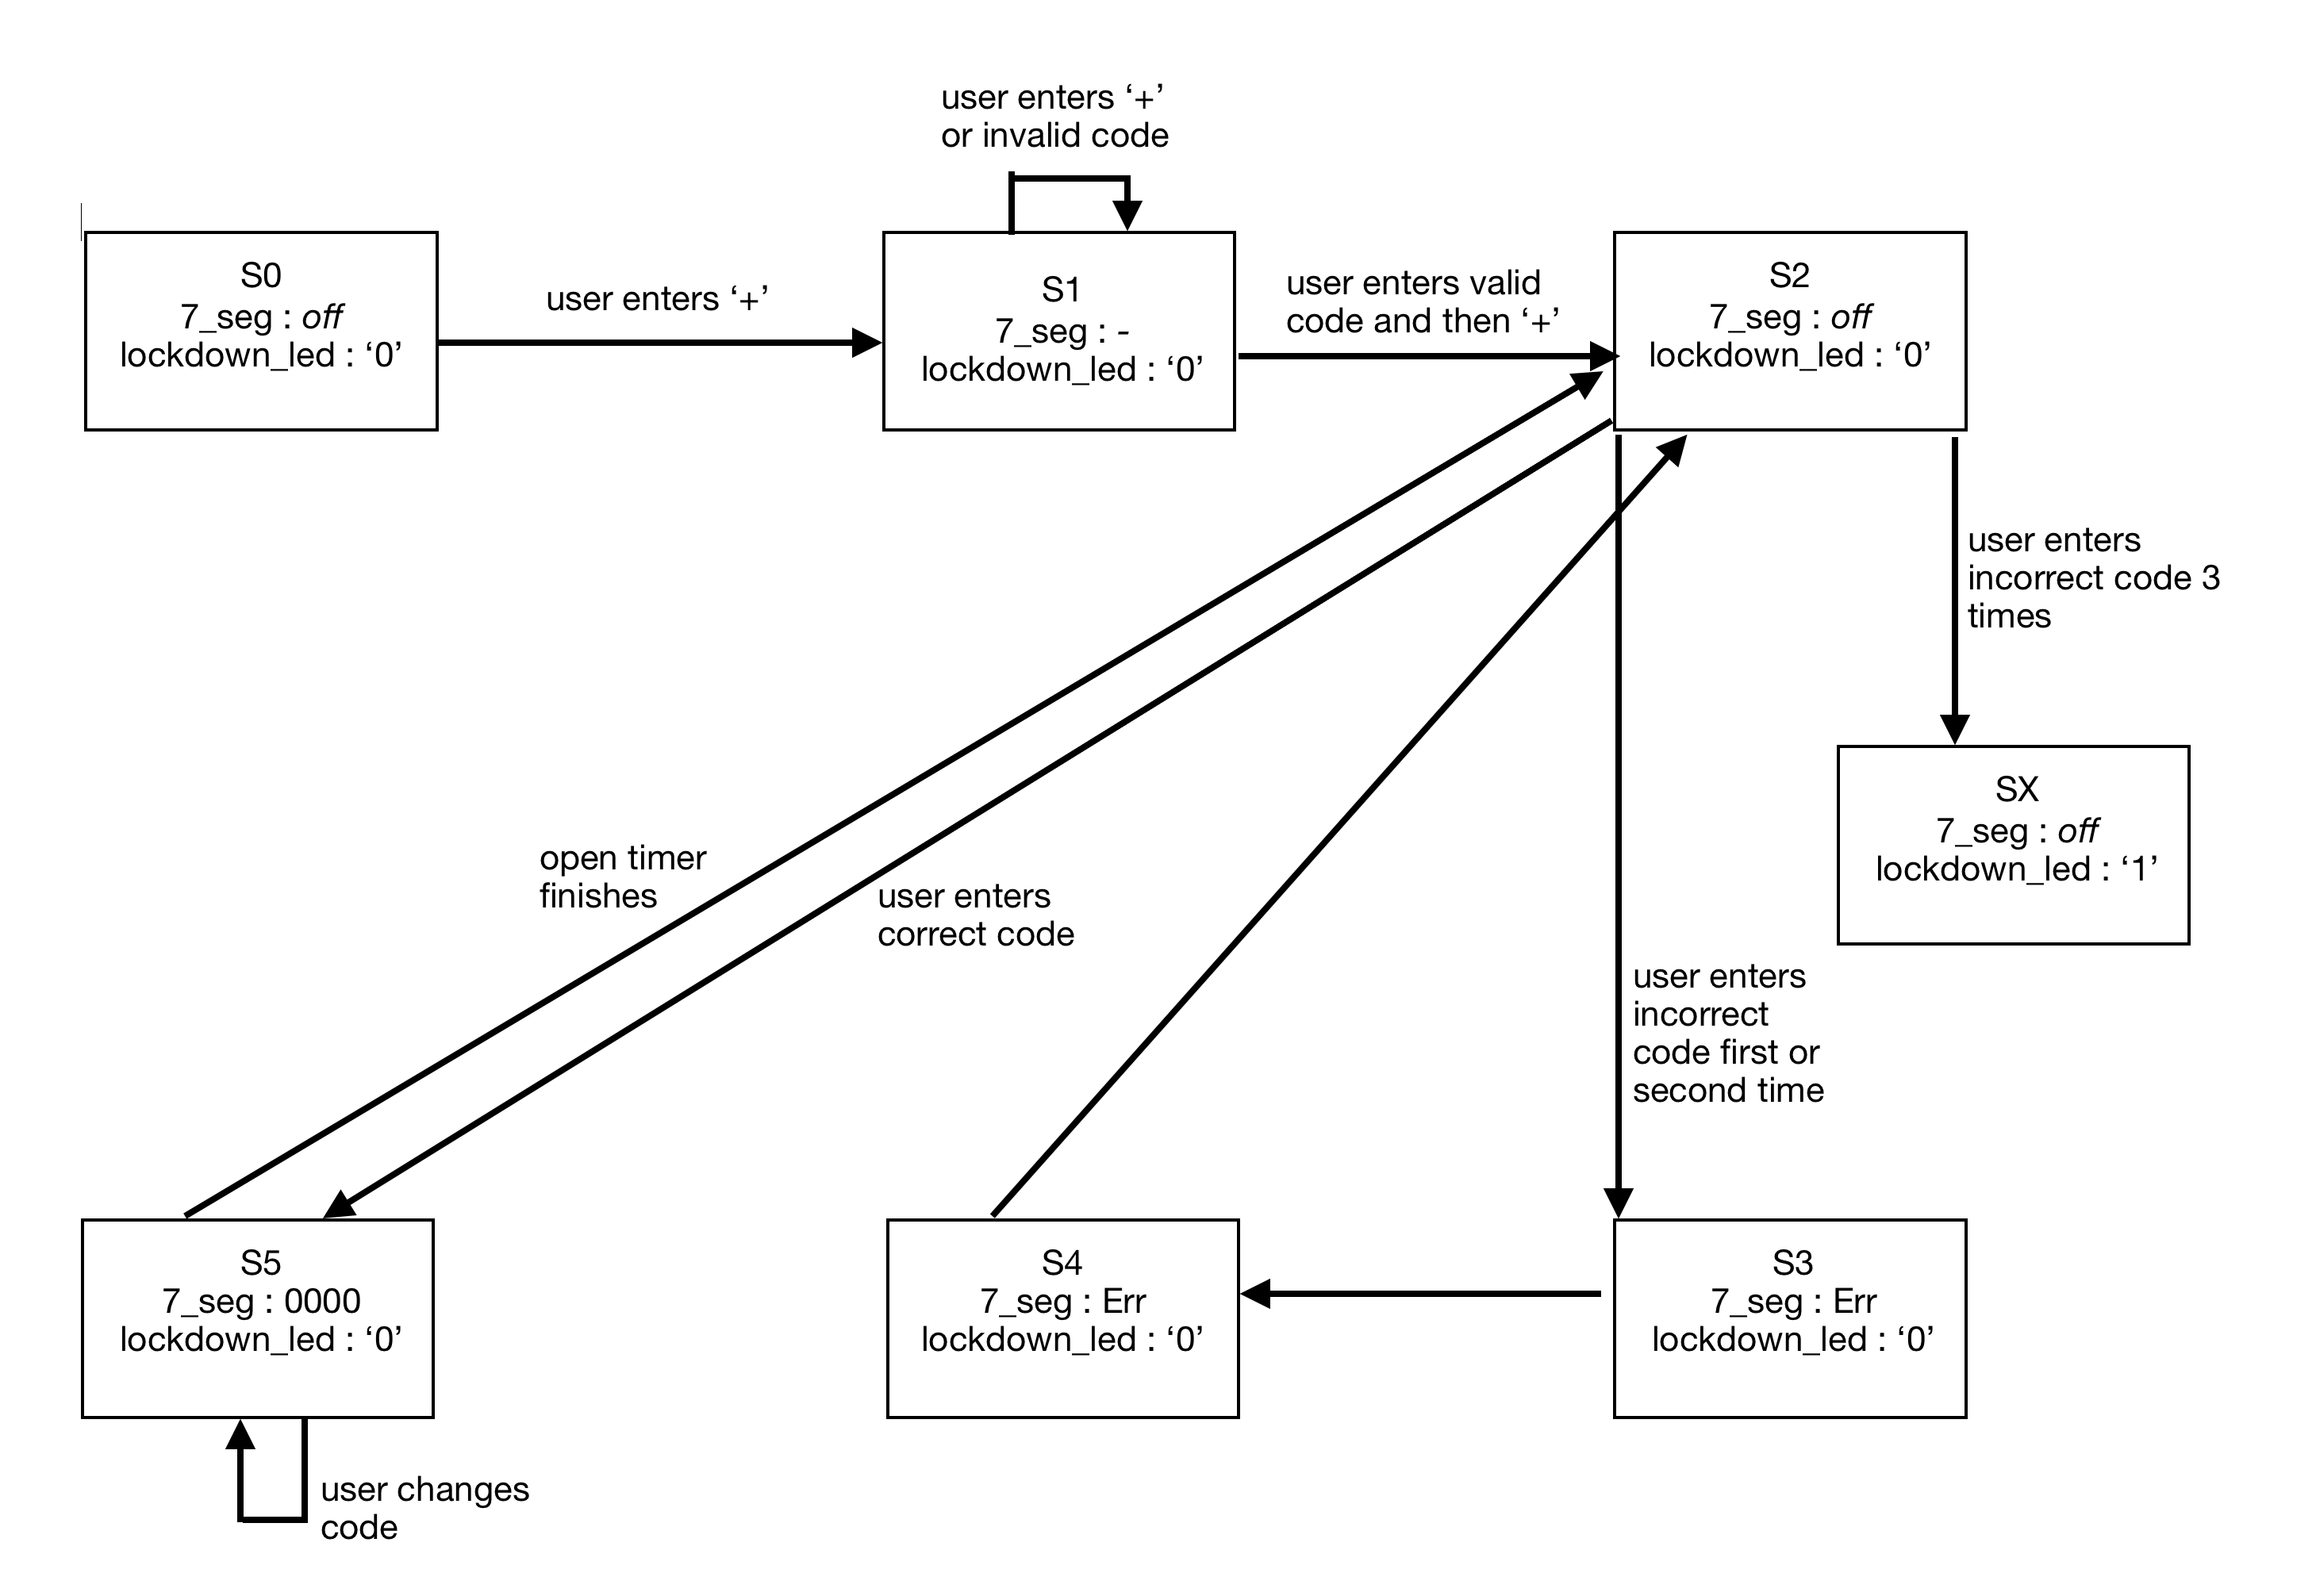
\includegraphics[width = \textwidth]{./img/statemachine.png}
	\caption{\label{fig:statemachine}System State Diagram}
\end{center}
\end{figure}

\section{Functional Specification}

\subsection{Initial Setup}

Initially, the system will have no code programmed. The user may program a code by pressing '+' to enter set mode. The user should then enter a 6-digit numeric code on the keypad and then press the '+' button again. This will exit set mode and save the code.

If the user enters more or less than 6 digits, or any non-numeric characters, the '+' key will cause the currently entered code to be cleared so the user may start setting again. If the code is cleared in this way, the 7-segment display should read "clr".

\subsection{Unlocking the Lock}

The keypad will be read every 0.25 seconds. The user should enter 6 numeric characters. As each character is entered,  it will be displayed on the least significant 7-segment display. After 6 characters are read, the system will display "0000" on the 7-segment displays if the correct code was entered, and "Err" if it was not.

The lock will remain unlocked for 15 seconds, and then the message will disappear and the system will be locked.

\subsection{Changing the Code}

To change the code after initial setup, the user must first enter the code. Then, while "OPEN" is displayed, press the '+' button to enter set mode.

Then, enter a 6-digit numeric code on the keypad and press the '+' button again. This will exit set mode and save the code.

If the user enters more or less than 6 digits, or any non-numeric characters, the '+' key will cause the currently entered code to be cleared so the user may start again. If the code is cleared in this way, the 7-segment display should read "clr".

\subsection{Display Timeout}

All messages on the 7-segment display, except for the "OPEN" message, will disappear after 2 seconds, or until a new character is entered, whichever comes first.

\subsection{Code Input Timeout}

If less then 6 digits are entered, they will be cleared after 20 seconds of no input from the user.

\subsection{Lockdown Mode}

If the incorrect code is entered 3 time, the system will enter lockdown mode. This will activate an LED indicator and the system will not unlock until its power is cycled.

\section{Development}

\subsection{Timer and Output Controller}

Development for this project began with developing the timer modules and the output  controller that would run the 7-segment displays. This section gave me the opportunity for one of my favorite achievements, successfully implementing multiple digits in the seven-segment display, utilizing some basic code to adapt to my needs \cite{sevseg}. One exciting accomplishment from this portion of development was learning how to ensure that a certain amount of time had passed without using a wait statement, as there were unavailable in the types of processes I was using.

\subsection{Finite State Machine}

Next I developed the finite state machine. This part became more difficult as each state in Figure \ref{fig:statemachine} actually has a subset of its own operations. A quick sketch of the in-depth state machine is provided in Figure \ref{fig:detstatemachine}. I now believe it was unwise to develop the state machine before having a way to receive my input from the user. Leaving this integration to last was the most significant challenge that I faced in this project. Additionally, designing this state machine to work well with an ILA or some other sort of debugging from the beginning would've allowed me to integrate the system more successfully.

\begin{figure}[H]
\begin{center}
	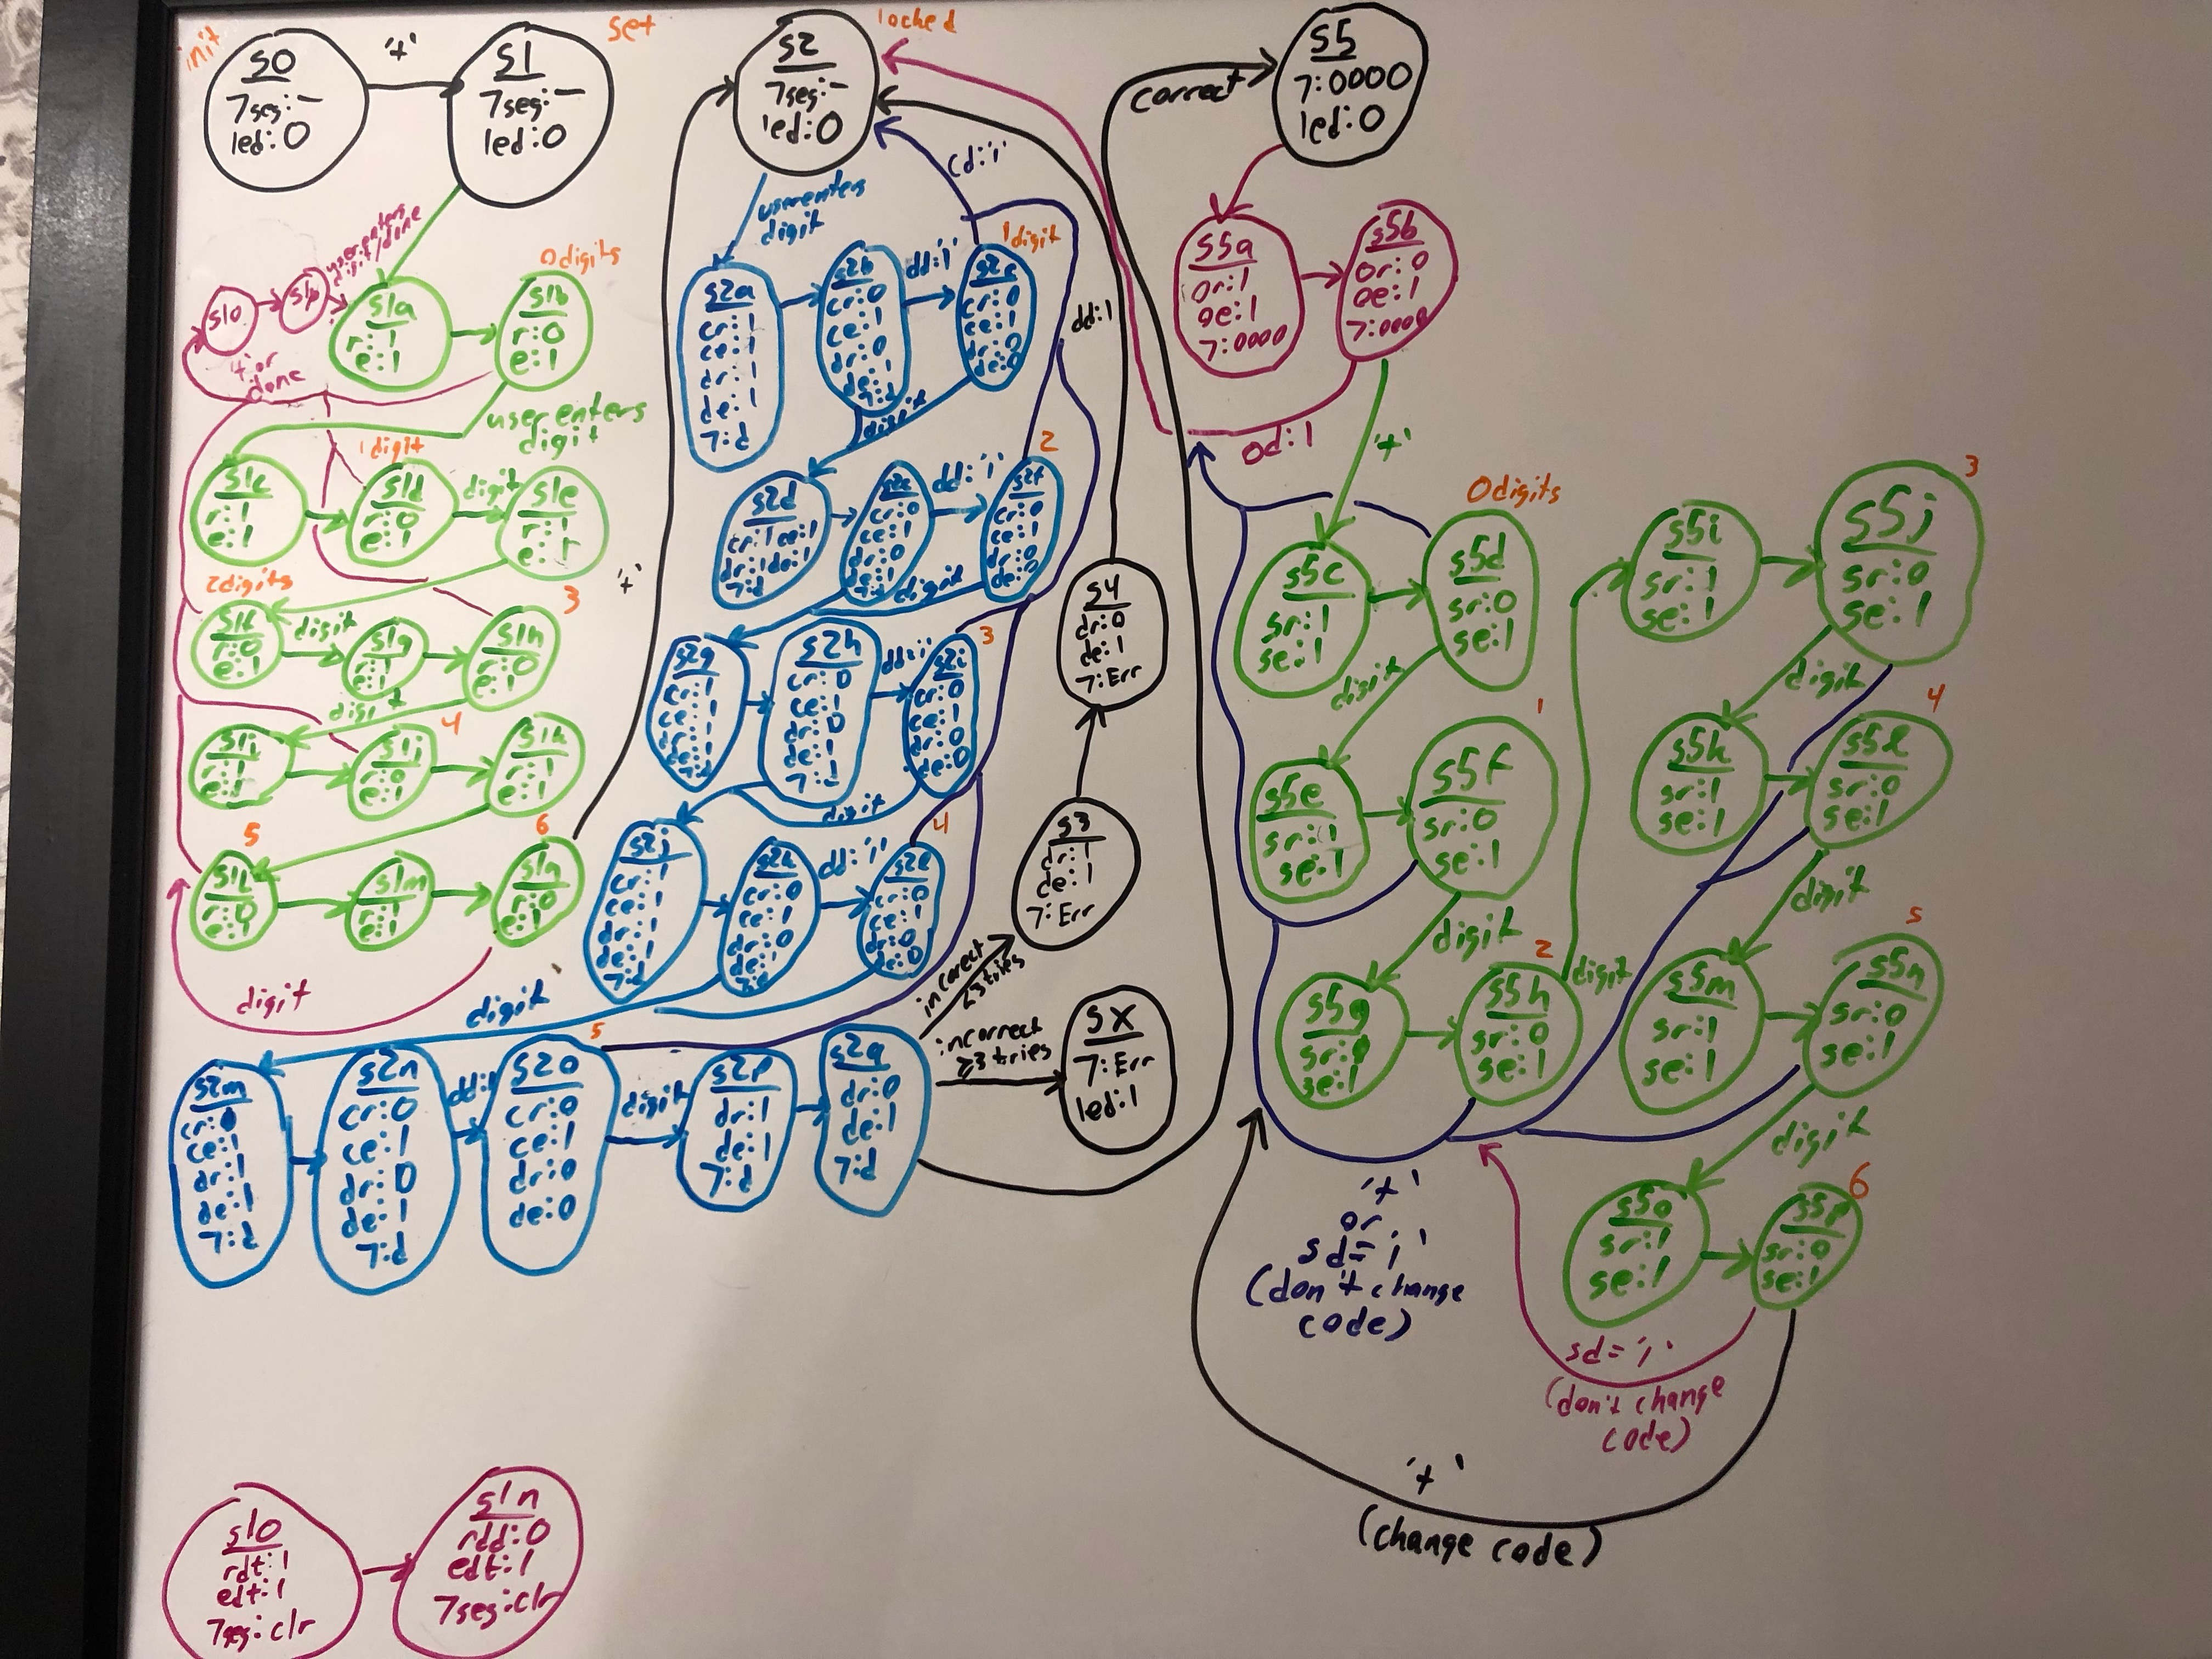
\includegraphics[width=\textwidth]{./img/detailstatemachine.jpg}
	\caption{\label{fig:detstatemachine}}
\end{center}
\end{figure}



\subsection{Input Controller}

Developing the input controller was another exciting accomplishment. It was quite difficult to ensure that the input would return to a non-input state quickly and smoothly enough to satisfy my input requirements. Bascially, it had to only show the input for the time of 1 state on my state machine so that I wouldn't accidentally provide the same input twice. As a starting point for this part of development, I found some tutorials from Digilent that were quite useful \cite{ps2}.

\subsection{System Integration}

My biggest failure in system integration was failing to prepare these modules ahead of time to be examined by ILAs. Basically, I worked for about a week to integrate this system, and realized relatively early I needed to integrate the ILA IP. However, as I set up several of my modules to be accessible by ILAs in the ways I wanted, I began to have synthesis errors that I just couldn't find a solution for related to signals with multiple drivers. Because I was unable to identify these issues, I was not able to complete a working system.

\section{Conclusion}

In conclusion, I found that my entire approach direction to this project led to it being incomplete at the due date. In the future, I should acquire input from the user first, and I should make each module testable the first time it is created. I faced the following pitfalls while working on this projects:

\begin{itemize}
	\item Troubleshooting with the ILA and testbenches
	\item System integration
\end{itemize}

However, I did learn quite a bit and had some major accomplishments during this project. Those accomplishments were:

\begin{itemize}
	\item Processing PS/2 Input for the first time
	\item Figuring out how to time operations without using wait statements
	\item Driving multiple digits of a seven segment display
\end{itemize}

\pagebreak

\textbf{Appendices}

\begin{appendices}

\section{Source Code}

\subsection{Top Level Module}

\begin{lstlisting}[language=VHDL]
library IEEE;
use IEEE.STD_LOGIC_1164.ALL;

entity digital_lock is
  port(ps2_data, ps2_clk, clk, reset : in std_logic;
    seven_seg_data : out std_logic_vector(11 downto 0);
    lockout_led : out std_logic;
    med_clk_led : out std_logic);
end entity digital_lock;

architecture digital_lock_arch of digital_lock is

  -- Signals for clock divider
  signal start_timer : std_logic := '0';
  signal fast_clk, med_clk, slow_clk, slow_clk_led : std_logic;

  -- Signals for input controller
  signal ps2_code_new : std_logic;
  signal ps2_code : std_logic_vector(3 downto 0);

  -- Signals for output controller
  signal display_cmd : std_logic_vector(3 downto 0);
  signal seven_seg_sig : std_logic_vector(11 downto 0);
  signal lockout_led_sig : std_logic;

  -- Signals for code timeout timer
  signal enable_code, reset_code : std_logic;
  signal code_timeout : std_logic;

  -- Signals for display timeout timer
  signal enable_display, reset_display : std_logic;
  signal display_timeout : std_logic;

  -- Signals for open timeout timer
  signal enable_open, reset_open : std_logic;
  signal open_timeout : std_logic;

  -- Signals for set timeout timer
  signal enable_set, reset_set : std_logic;
  signal set_timeout : std_logic;

  component clock_divider is
    port(clk : in std_logic;
         start_timer : in std_logic;
         FastClock,MediumClock,SlowClock, led0 : out std_logic);
  end component clock_divider;

  component input_controller is
    port(clk, ps2_clk, ps2_data : in std_logic;
      ps2_code_new : out std_logic;
      ps2_code     : out std_logic_vector(3 downto 0));
  end component input_controller;

  component output_controller is
    port(display : in std_logic_vector(3 downto 0);
      clk : in std_logic;
      lockout_led : out std_logic;
      seven_seg : out std_logic_vector(11 downto 0));
  end component output_controller;

  component code_timeout_timer is
    port(enable, reset, one_hz_clk : in std_logic;
      done : out std_logic);
  end component code_timeout_timer;

  component display_timeout_timer is
    port(enable, reset, one_hz_clk : in std_logic;
      done : out std_logic);
  end component display_timeout_timer;

  component open_timeout_timer is
    port(enable, reset, one_hz_clk : in std_logic;
      done : out std_logic);
  end component open_timeout_timer;

  component set_timeout_timer is
    port(enable, reset, one_hz_clk : in std_logic;
      done : out std_logic);
  end component set_timeout_timer;

  component main is
    port(sys_clk, clk, reset : in std_logic;
      cmd : in std_logic_vector(3 downto 0);
      code_timeout, set_timeout, open_timeout, display_timeout : in std_logic;
      enable_code, reset_code, enable_set, reset_set, enable_open, reset_open,
      enable_display, reset_display : out std_logic;
      lockout_led : out std_logic;
      display_cmd : out std_logic_vector(3 downto 0));
  end component main;

begin
  ic : input_controller port map(clk, ps2_clk, ps2_data, ps2_code_new, ps2_code);
  clk_div : clock_divider port map(clk, start_timer, fast_clk, med_clk,
  		 slow_clk, slow_clk_led);
  oc : output_controller port map(display_cmd, clk, lockout_led_sig, 
  		seven_seg_sig);
  code_timer : code_timeout_timer port map(enable_code, reset_code, 
  		slow_clk, code_timeout);
  display_timer : display_timeout_timer port map(enable_display, 
  		reset_display, slow_clk, display_timeout);
  open_timer : open_timeout_timer port map(enable_open, reset_open, 
  		slow_clk, open_timeout);
  set_timer : set_timeout_timer port map(enable_set, reset_set, slow_clk,
  		 set_timeout);
  main_fsm : main port map(clk, med_clk, reset, ps2_code, code_timeout, 
  		set_timeout, open_timeout, display_timeout, enable_code,
  		reset_code,  enable_set, reset_set, enable_open, reset_open, 
  		enable_display, reset_display, lockout_led, display_cmd);

  lockout_led <= lockout_led_sig;
  seven_seg_data <= seven_seg_sig;
  med_clk_led <= med_clk;
end architecture digital_lock_arch;
\end{lstlisting}

\subsection{Main State Machine}

\begin{lstlisting}[language=VHDL]
library IEEE;
use IEEE.STD_LOGIC_1164.ALL;
use IEEE.NUMERIC_STD.ALL;

entity main is
  port (
    sys_clk, clk, reset : in std_logic;
    -- values for cmd
    -- 0, 1, 2, 3, 4, 5, 6, 7, 8, 9, +, nothing
    cmd : in std_logic_vector(3 downto 0);
    code_timeout, set_timeout, open_timeout, display_timeout : in std_logic;
    enable_code, reset_code, enable_set, reset_set, enable_open, reset_open, 
    		enable_display, reset_display : out std_logic;
    lockout_led : out std_logic;
    -- values for display_cmd
    -- 0 - 9 : value of BCD
    -- 1010 : '0000'
    -- 1011 : 'Clr'
    -- 1100 : "Err"
    -- 1101 : lockout
    -- 1111 : display off
    display_cmd : out std_logic_vector(3 downto 0));
end entity main;

architecture main_behavior of main is
  TYPE State_Type IS (s0, s1, s1a, s1b, s1c, s1d, s1e, s1f, s1g, s1h, s1i,
    s1j, s1k, s1l, s1m, s1n, s1o, s1p, s2, s2a, s2b, s2c, s2d, s2e, s2f,
    s2g, s2h, s2i, s2j, s2k, s2l, s2m, s2n, s2o, s2p, s2q, s3, s4, s5,
    s5a, s5b, s5c, s5d, s5e, s5f, s5g, s5h, s5i, s5j, s5k, s5l, s5m, s5n,
    s5o, s5p, sX);
  signal current_state : State_Type := s0;
  signal next_state : State_Type;

  --This signal holds the number of attempts, 0-3
  signal attempts : std_logic_vector (1 downto 0) := "00";

  -- These six signals make up the code for the lock
  -- code_five is most significant digit
  signal code_five : std_logic_vector(3 downto 0) := "0000";
  signal code_four : std_logic_vector(3 downto 0) := "0000";
  signal code_three : std_logic_vector(3 downto 0) := "0000";
  signal code_two : std_logic_vector(3 downto 0) := "0000";
  signal code_one : std_logic_vector(3 downto 0) := "0000";
  signal code_zero : std_logic_vector(3 downto 0) := "0000";

  -- These six signals hold a new code that has not yet been saved
  -- new_code_five is most significant digit
  signal new_code_five : std_logic_vector(3 downto 0) := "0000";
  signal new_code_four : std_logic_vector(3 downto 0) := "0000";
  signal new_code_three : std_logic_vector(3 downto 0) := "0000";
  signal new_code_two : std_logic_vector(3 downto 0) := "0000";
  signal new_code_one : std_logic_vector(3 downto 0) := "0000";
  signal new_code_zero : std_logic_vector(3 downto 0) := "0000";

  -- These six signal hold the users entry for the lock
  -- code_entry_five is most significant digit
  signal code_entry_five : std_logic_vector(3 downto 0) := "0000";
  signal code_entry_four : std_logic_vector(3 downto 0) := "0000";
  signal code_entry_three : std_logic_vector(3 downto 0) := "0000";
  signal code_entry_two : std_logic_vector(3 downto 0) := "0000";
  signal code_entry_one : std_logic_vector(3 downto 0) := "0000";
  signal code_entry_zero : std_logic_vector(3 downto 0) := "0000";

begin

  process(clk,reset)
  begin
    if(reset = '1') then
      next_state <= s0;
    elsif(clk'event and clk = '1') then
      case current_state is
        when s0 =>
          if(cmd = "1010") then
            next_state <= s1;
          else
            next_state <= s0;
          end if;
        when s1 =>
          next_state <= s1a;
        when s1a =>
          next_state <= s1b;
        when s1b =>
          if(cmd /= "1011") then
            next_state <= s1c;
            new_code_five <= cmd;
          elsif((cmd = "1010") or (set_timeout = '1')) then
            next_state <= s1o;
          else
            next_state <= s1b;
          end if;
        when s1c =>
          next_state <= s1d;
        when s1d =>
          if(cmd /= "1011") then
            next_state <= s1e;
            new_code_four <= cmd;
          elsif((cmd = "1010") or (set_timeout = '1')) then
            next_state <= s1o;
          else
            next_state <= s1d;
          end if;
        when s1e =>
          next_state <= s1f;
        when s1f =>
          if(cmd /= "1011") then
            next_state <= s1g;
            new_code_three <= cmd;
          elsif((cmd = "1010") or (set_timeout = '1')) then
            next_state <= s1o;
          else
            next_state <= s1f;
          end if;
        when s1g =>
          next_state <= s1h;
        when s1h =>
          if(cmd /= "1011") then
            next_state <= s1i;
            new_code_two <= cmd;
          elsif((cmd = "1010") or (set_timeout = '1')) then
            next_state <= s1o;
          else
            next_state <= s2h;
          end if;
        when s1i =>
          next_state <= s1j;
        when s1j =>
          if(cmd /= "1011") then
            next_state <= s1k;
            new_code_one <= cmd;
          elsif((cmd = "1010") or (set_timeout = '1')) then
            next_state <= s1o;
          end if;
        when s1k =>
          next_state <= s1l;
        when s1l =>
          if(cmd /= "1011") then
            next_state <= s1m;
            new_code_zero <= cmd;
          elsif((cmd = "1010") or (set_timeout = '1')) then
            next_state <= s1o;
          else
            next_state <= s1l;
          end if;
        when s1m =>
          next_state <= s1n;
        when s1n =>
          if(cmd = "1010") then
            next_state <= s2;
            code_five <= new_code_five;
            code_four <= new_code_four;
            code_three <= new_code_three;
            code_two <= new_code_two;
            code_one <= new_code_one;
            code_zero <= new_code_zero;
          elsif((cmd /= "1011") or (set_timeout = '1')) then
            next_state <= s1o;
          else
            next_state <= s1n;
          end if;
        when s1o =>
          next_state <= s1p;
        when s1p =>
          if((cmd /= "1011") or (display_timeout = '1')) then
            next_state <= s1a;
          else
            next_state <= s1p;
          end if;
        when s2 =>
          if(cmd /= "1011") then
            code_entry_five <= cmd;
            next_state <= s2a;
          else
            next_state <= s2;
          end if;
        when s2a =>
          next_state <= s2b;
        when s2b =>
          if(cmd /= "1011") then
            code_entry_four <= cmd;
            next_state <= s2d;
          elsif(display_timeout = '1') then
            next_state <= s2c;
          else
            next_state <= s2b;
          end if;
        when s2c =>
          if(code_timeout = '1') then
            next_state <= s2;
          elsif(cmd /="1011") then
            code_entry_four <= cmd;
            next_state <= s2d;
          else
            next_state <= s2c;
          end if;
        when s2d =>
          next_state <= s2e;
        when s2e =>
          if(cmd /= "1011") then
            code_entry_three <= cmd;
            next_state <= s2g;
          elsif(display_timeout = '1') then
            next_state <= s2f;
          else
            next_state <= s2e;
          end if;
        when s2f =>
          if(code_timeout = '1') then
            next_state <= s2;
          elsif(cmd /="1011") then
            code_entry_three <= cmd;
            next_state <= s2d;
          else
            next_state <= s2f;
          end if;
        when s2g =>
          next_state <= s2h;
        when s2h =>
          if(cmd /= "1011") then
            code_entry_two <= cmd;
            next_state <= s2j;
          elsif(display_timeout = '1') then
            next_state <= s2i;
          else
            next_state <= s2h;
          end if;
        when s2i =>
          if(code_timeout = '1') then
            next_state <= s2;
          elsif(cmd /="1011") then
            code_entry_two <= cmd;
            next_state <= s2j;
          else
            next_state <= s2i;
          end if;
        when s2j =>
          next_state <= s2k;
        when s2k =>
          if(cmd /= "1011") then
            code_entry_one <= cmd;
            next_state <= s2m;
          elsif(display_timeout = '1') then
            next_state <= s2l;
          else
            next_state <= s2k;
          end if;
        when s2l =>
          if(code_timeout = '1') then
            next_state <= s2;
          elsif(cmd /="1011") then
            code_entry_one <= cmd;
            next_state <= s2m;
          else
            next_state <= s2l;
          end if;
        when s2m =>
          next_state <= s2n;
        when s2n =>
          if(cmd /= "1011") then
            code_entry_zero <= cmd;
            next_state <= s2p;
          elsif(display_timeout = '1') then
            next_state <= s2o;
          else
            next_state <= s2n;
          end if;
        when s2o =>
          if(code_timeout = '1') then
            next_state <= s2;
          elsif(cmd /="1011") then
            code_entry_zero <= cmd;
            next_state <= s2p;
          else
            next_state <= s2o;
          end if;
        when s2p =>
          next_state <= s2q;
        when s2q =>
          if((code_entry_five /= code_five) or
          (code_entry_four /= code_four) or
          (code_entry_three /= code_three) or
          (code_entry_two /= code_two) or
          (code_entry_one /= code_one) or
          (code_entry_zero /= code_zero)) then
            if(attempts < "11") then
              next_state <= s3;
              attempts <= std_logic_vector(unsigned(attempts) + 1);
            else
              next_state <= sX;
            end if;
          else
            next_state <= s5;
          end if;
        when s3 =>
          next_state <= s4;
        when s4 =>
          if(display_timeout = '1') then
            next_state <= s2;
          end if;
        when s5 =>
          next_state <= s5a;
        when s5a =>
          next_state <= s5b;
        when s5b =>
          if(open_timeout = '1') then
            next_state <= s2;
          elsif(cmd = "1010") then
            next_state <= s5c;
          else
            next_state <= s5b;
          end if;
        when s5c =>
          next_state <= s5d;
        when s5d =>
          if(cmd /= "1011") then
            new_code_five <= cmd;
            next_state <= s5e;
          elsif((cmd = "1010") or (set_timeout = '1')) then
            next_state <= s2;
          else
            next_state <= s5d;
          end if;
        when s5e =>
          next_state <= s5f;
        when s5f =>
          if(cmd /= "1011") then
            new_code_four <= cmd;
            next_state <= s5g;
          elsif((cmd = "1010") or (set_timeout = '1')) then
            next_state <= s2;
          else
            next_state <= s5f;
          end if;
        when s5g =>
          next_state <= s5h;
        when s5h =>
          if(cmd /= "1011") then
            new_code_three <= cmd;
            next_state <= s5i;
          elsif((cmd = "1010") or (set_timeout = '1')) then
            next_state <= s2;
          else 
            next_state <= s5h;
          end if;
        when s5i =>
          next_state <= s5j;
        when s5j =>
          if(cmd /= "1011") then
            new_code_two <= cmd;
            next_state <= s5k;
          elsif((cmd = "1010") or (set_timeout = '1')) then
            next_state <= s2;
          else
            next_state <= s5j;
          end if;
        when s5k =>
          next_state <= s5l;
        when s5l =>
          if(cmd /= "1011") then
            new_code_one <= cmd;
            next_state <= s5m;
          elsif((cmd = "1010") or (set_timeout = '1')) then
            next_state <= s2;
          else
            next_state <= s5l;
          end if;
        when s5m =>
          next_state <= s5n;
        when s5n =>
          if(cmd /= "1011") then
            new_code_zero <= cmd;
            next_state <= s5o;
          elsif((cmd = "1010") or (set_timeout = '1')) then
            next_state <= s2;
          else
            next_state <= s5n;
          end if;
        when s5o =>
          next_state <= s5p;
        when s5p =>
          if(cmd = "1010") then
            code_five <= new_code_five;
            code_four <= new_code_four;
            code_three <= new_code_three;
            code_two <= new_code_two;
            code_one <= new_code_one;
            code_zero <= new_code_zero;
            next_state <= s2;
          elsif(set_timeout = '1') then
            next_state <= s2;
          else
            next_state <= s5p;
          end if;
        when sX =>
          next_state <= sX;
      end case;
    end if;
  end process;
  process(current_state)
  begin
    case(current_state) is
      when s0 =>
        display_cmd <= "1111";
        lockout_led <= '0';
      when s1 =>
        display_cmd <= "1111";
        lockout_led <= '0';
      when s1a =>
        display_cmd <= "1111";
        reset_set <= '1';
        enable_set <= '1';
      when s1b =>
        reset_set <= '0';
        enable_set <= '1';
      when s1c =>
        reset_set <= '1';
        enable_set <= '1';
      when s1d =>
        reset_set <= '0';
        enable_set <= '1';
      when s1e =>
        reset_set <= '1';
        enable_set <= '1';
      when s1f =>
        reset_set <= '0';
        enable_set <= '1';
      when s1g =>
        reset_set <= '1';
        enable_set <= '1';
      when s1h =>
        reset_set <= '0';
        enable_set <= '1';
      when s1i =>
        reset_set <= '1';
        enable_set <= '1';
      when s1j =>
        reset_set <= '0';
        enable_set <= '1';
      when s1k =>
        reset_set <= '1';
        enable_set <= '1';
      when s1l =>
        reset_set <= '0';
        enable_set <= '1';
      when s1m =>
        reset_set <= '1';
        enable_set <= '1';
      when s1n =>
        reset_set <= '0';
        enable_set <= '1';
      when s1o =>
        enable_set <= '0';
        reset_display <= '1';
        enable_display <= '1';
        display_cmd <= "1011";
      when s1p =>
        reset_display <= '0';
        enable_display <= '1';
        display_cmd <= "1011";
      when s2 =>
        enable_set <= '0';
        enable_open <= '0';
        enable_display <= '0';
        display_cmd <= "1111";
        lockout_led <= '0';
      when s2a =>
        reset_code <= '1';
        enable_code <= '1';
        reset_display <= '1';
        enable_display <= '1';
        display_cmd <= cmd;
      when s2b =>
        reset_code <= '0';
        enable_code <= '1';
        reset_display <= '0';
        enable_display <= '1';
        display_cmd <= cmd;
      when s2c =>
        reset_code <= '0';
        enable_code <= '1';
        reset_display <= '0';
        enable_display <= '0';
        display_cmd <= cmd;
      when s2d =>
        reset_code <= '1';
        enable_code <= '1';
        reset_display <= '1';
        enable_display <= '1';
        display_cmd <= cmd;
      when s2e =>
        reset_code <= '0';
        enable_code <= '1';
        reset_display <= '0';
        enable_display <= '1';
        display_cmd <= cmd;
      when s2f =>
        reset_code <= '0';
        enable_code <= '1';
        reset_display <= '0';
        enable_display <= '0';
        display_cmd <= cmd;
      when s2g =>
        reset_code <= '1';
        enable_code <= '1';
        reset_display <= '1';
        enable_display <= '1';
        display_cmd <= cmd;
      when s2h =>
        reset_code <= '0';
        enable_code <= '1';
        reset_display <= '0';
        enable_display <= '1';
        display_cmd <= cmd;
      when s2i =>
        reset_code <= '0';
        enable_code <= '1';
        reset_display <= '0';
        enable_display <= '0';
        display_cmd <= cmd;
      when s2j =>
        reset_code <= '1';
        enable_code <= '1';
        reset_display <= '1';
        enable_display <= '1';
        display_cmd <= cmd;
      when s2k =>
        reset_code <= '0';
        enable_code <= '1';
        reset_display <= '0';
        enable_display <= '1';
        display_cmd <= cmd;
      when s2l =>
        reset_code <= '0';
        enable_code <= '1';
        reset_display <= '0';
        enable_display <= '0';
        display_cmd <= cmd;
      when s2m =>
        reset_code <= '1';
        enable_code <= '1';
        reset_display <= '1';
        enable_display <= '1';
        display_cmd <= cmd;
      when s2n =>
        reset_code <= '0';
        enable_code <= '1';
        reset_display <= '0';
        enable_display <= '1';
        display_cmd <= cmd;
      when s2o =>
        reset_code <= '0';
        enable_code <= '1';
        reset_display <= '0';
        enable_display <= '0';
        display_cmd <= cmd;
      when s2p =>
        reset_code <= '0';
        enable_code <= '0';
        reset_display <= '1';
        enable_display <= '1';
        display_cmd <= cmd;
      when s2q =>
        reset_display <= '0';
        enable_display <= '1';
        display_cmd <= cmd;
      when s3 =>
        reset_display <= '1';
        enable_display <= '1';
        display_cmd <= "1100";
      when s4 =>
        reset_display <= '0';
        enable_display <= '1';
        display_cmd <= "1100";
      when s5 =>
        display_cmd <= "1010";
        lockout_led <= '0';
      when s5a =>
        reset_open <= '1';
        enable_open <= '1';
        display_cmd <= "1010";
      when s5b =>
        reset_open <= '0';
        enable_open <= '1';
        display_cmd <= "1010";
      when s5c =>
        reset_set <= '1';
        enable_set <= '1';
      when s5d =>
        reset_set <= '0';
        enable_set <= '1';
      when s5e =>
        reset_set <= '1';
        enable_set <= '1';
      when s5f =>
        reset_set <= '0';
        enable_set <= '1';
      when s5g =>
        reset_set <= '1';
        enable_set <= '1';
      when s5h =>
        reset_set <= '0';
        enable_set <= '1';
      when s5i =>
        reset_set <= '1';
        enable_set <= '1';
      when s5j =>
        reset_set <= '0';
        enable_set <= '1';
      when s5k =>
        reset_set <= '1';
        enable_set <= '1';
      when s5l =>
        reset_set <= '0';
        enable_set <= '1';
      when s5m =>
        reset_set <= '1';
        enable_set <= '1';
      when s5n =>
        reset_set <= '0';
        enable_set <= '1';
      when s5o =>
        reset_set <= '1';
        enable_set <= '1';
      when s5p =>
        reset_set <= '0';
        enable_set <= '1';
      when sx =>
        display_cmd <= "1101";
        lockout_led <= '1';
    end case;
  end process;
  current_state <= next_state;
end architecture main_behavior;

\end{lstlisting}

\subsection{Input Controller}

\begin{lstlisting}[language=VHDL]
library IEEE;
use IEEE.STD_LOGIC_1164.ALL;
use IEEE.NUMERIC_STD.ALL;

entity input_controller is
  generic(
    clk_freq : integer := 50_000_000;
    debounce_counter_size : integer := 8);
  port(
    clk          : in  std_logic;
    ps2_clk      : in  std_logic;
    ps2_data     : in  std_logic;
    ps2_code_new : out std_logic;
    ps2_code     : out std_logic_vector(3 downto 0));
end input_controller;

architecture input_controller_arch of input_controller is
  signal sync_ffs     : std_logic_vector(1 downto 0);
  signal ps2_clk_int  : std_logic;
  signal ps2_data_int : std_logic;
  signal ps2_word     : std_logic_vector(10 downto 0);
  signal error        : std_logic;
  signal count_idle   : integer range 0 to clk_freq/18_000;
  signal ps2_code_sig : std_logic_vector(7 downto 0);
  signal ps2_code_timeout : std_logic_vector(27 downto 0) 
  		:= "0000000000000000000000000000";
  signal ps2_code_timeout_comparator : std_logic_vector (1 downto 0);


  -- debouncing PS2 input signals
  component debouncer is
    generic(
      counter_size : integer); --debounce period (in seconds) 
    port(
      clk    : in  std_logic;  --input clock
      button : in  std_logic;  --input signal to be debounced
      result : out STD_LOGIC); --debounced signal
  end component;
begin

  -- synchronizer flip-flops
  process(clk)
  begin
    if(clk'event and clk = '1') then
      sync_ffs(0) <= ps2_clk;
      sync_ffs(1) <= ps2_data;
    end if;
  end process;

  --debounce PS2 input signals
  debounce_ps2_clk: debouncer
    generic map(counter_size => debounce_counter_size)
    port map(clk => clk, button => sync_ffs(0), result => ps2_clk_int);
  debounce_ps2_data: debouncer
    generic map(counter_size => debounce_counter_size)
    port map(clk => clk, button => sync_ffs(1), result => ps2_data_int);

  --input PS2 data
  process(ps2_clk_int)
  begin
    if(ps2_code_timeout_comparator >= "01") then
        ps2_word <= "00000000000";
    elsif(ps2_clk_int'event and ps2_clk_int = '0') then
      ps2_word <= ps2_data_int & ps2_word(10 downto 1);
    end if;
  end process;

  --verify that parity, start, and stop bits are all correct
  error <= not (not ps2_word(0) and ps2_word(10) 
  	   and (ps2_word(9) xor ps2_word(8) xor
        ps2_word(7) xor ps2_word(6) xor ps2_word(5) 
        xor ps2_word(4) xor ps2_word(3) xor
        ps2_word(2) xor ps2_word(1)));

  --determine if PS2 port is idle and output result
  process(clk)
  begin
    if(clk'event and clk = '1') then

      if(ps2_clk_int = '0') then
        count_idle <= 0;
      elsif(count_idle /= clk_freq/18_000) then
          count_idle <= count_idle + 1;
      end if;

      if(count_idle = clk_freq/18_000 and error = '0') then
        ps2_code_new <= '1';
        ps2_code_sig <= ps2_word(8 downto 1);
      else
        ps2_code_new <= '0';
      end if;

    end if;
  end process;

  process(ps2_code_sig, ps2_code_timeout)
  begin
    if(ps2_code_timeout_comparator >= "01") then
      ps2_code <= "1011";
    else
      case ps2_word(8 downto 1) is
          when "01110000" =>
              ps2_code <= "0000";
          when "01101001" =>
              ps2_code <= "0001";
          when "01110010" =>
              ps2_code <= "0010";
          when "01111010" =>
              ps2_code <= "0011";
          when "01101011" =>
              ps2_code <= "0100";
          when "01110011" =>
              ps2_code <= "0101";
          when "01110100" =>
              ps2_code <= "0110";
          when "01101100" =>
              ps2_code <= "0111";
          when "01110101" =>
              ps2_code <= "1000";
          when "01111101" =>
              ps2_code <= "1001";
          when "01111001" =>
              ps2_code <= "1010";
          when others =>
              ps2_code <= "1011";
      end case;
    end if;
  end process;

  process(clk)
  begin
    if(clk'event and clk = '1') then
      ps2_code_timeout <= std_logic_vector(unsigned(ps2_code_timeout) + 1);
    end if;
    if(ps2_code_timeout_comparator >= "10") then
      ps2_code_timeout <= "0000000000000000000000000000";
    end if;
  end process;

  ps2_code_timeout_comparator <= ps2_code_timeout(27 downto 26);
end architecture input_controller_arch;

\end{lstlisting}

\subsection{Output Controller}

\begin{lstlisting}[language=VHDL]
library IEEE;
use IEEE.STD_LOGIC_1164.ALL;
use IEEE.NUMERIC_STD.ALL;

entity output_controller is
  port(display : in std_logic_vector(3 downto 0);
    clk : in std_logic;
    lockout_led : out std_logic;
    seven_seg : out std_logic_vector(11 downto 0));
end entity output_controller;

architecture output_behavior of output_controller is

  signal refresh_counter : std_logic_vector(19 downto 0);
  signal anode_counter : std_logic_vector(1 downto 0);
  signal display_one, display_two, display_three, 
  		display_four : std_logic_vector(7 downto 0);

begin

    -- Clock process for a 10.5ms refresh period
    process(clk)
    begin
        if(clk'event and clk = '1') then
            refresh_counter <= std_logic_vector(unsigned(refresh_counter) + 1);
        end if;
    end process;
    anode_counter <= refresh_counter(19 downto 18);
    process(anode_counter)
    begin
        case anode_counter is
        when "00" =>
            seven_seg(11 downto 8) <= "0111";
            seven_seg(7 downto 0) <= display_one;
        when "01" =>
            seven_seg(11 downto 8) <= "1011";
            seven_seg(7 downto 0) <= display_two;
        when "10" =>
            seven_seg(11 downto 8) <= "1101";
            seven_seg(7 downto 0) <= display_three;
        when "11" =>
            seven_seg(11 downto 8) <= "1110";
            seven_seg(7 downto 0) <= display_four;
        end case;
    end process;

    process(display)
        begin
            case display is
              when "0000" =>
                -- display '0'
                display_one <= "11111111";
                display_two <= "11111111";
                display_three <= "11111111";
                display_four <= "00000011";
                lockout_led <= '0';
              when "0001" =>
                -- display '1'
                display_one <= "11111111";
                display_two <= "11111111";
                display_three <= "11111111";
                display_four <= "10011111";
                lockout_led <= '0';
              when "0010" =>
                -- display '2'
                display_one <= "11111111";
                display_two <= "11111111";
                display_three <= "11111111";
                display_four <= "00100101";
                lockout_led <= '0';
              when "0011" =>
                -- display '3'
                display_one <= "11111111";
                display_two <= "11111111";
                display_three <= "11111111";
                display_four <= "00001101";
                lockout_led <= '0';
              when "0100" =>
                -- display '4'
                display_one <= "11111111";
                display_two <= "11111111";
                display_three <= "11111111";
                display_four <= "10011001";
                lockout_led <= '0';
              when "0101" =>
                -- display '5'
                display_one <= "11111111";
                display_two <= "11111111";
                display_three <= "11111111";
                display_four <= "01001001";
                lockout_led <= '0';
              when "0110" =>
                -- display '6'
                display_one <= "11111111";
                display_two <= "11111111";
                display_three <= "11111111";
                display_four <= "01000001";
                lockout_led <= '0';
              when "0111" =>
                -- display '7'
                display_one <= "11111111";
                display_two <= "11111111";
                display_three <= "11111111";
                display_four <= "00011111";
                lockout_led <= '0';
              when "1000" =>
                -- display '8'
                display_one <= "11111111";
                display_two <= "11111111";
                display_three <= "11111111";
                display_four <= "00000001";
                lockout_led <= '0';
              when "1001" =>
                -- display '9'
                display_one <= "11111111";
                display_two <= "11111111";
                display_three <= "11111111";
                display_four <= "00001001";
                lockout_led <= '0';
              when "1010" =>
                -- make display show "0000"
                display_one <= "00000011";
                display_two <= "00000011";
                display_three <= "00000011";
                display_four <= "00000011";
                lockout_led <= '0';
              when "1011" =>
                -- make display show "Clr"
                display_one <= "11111111";
                display_two <= "11100101";
                display_three <= "11110011";
                display_four <= "11110101";
                lockout_led <= '0';
              when "1100" =>
                -- make display show "err"
                display_one <= "11111111";
                display_two <= "01100001";
                display_three <= "11110101";
                display_four <= "11110101";
                lockout_led <= '0';
              when "1101" =>
                -- lockout led
                display_one <= "11111111";
                display_two <= "11111111";
                display_three <= "11111111";
                display_four <= "11111111";
                lockout_led <= '1';
              when others =>
                -- display off
                display_one <= "11111111";
                display_two <= "11111111";
                display_three <= "11111111";
                display_four <= "11111111";
                lockout_led <= '0';
            end case;
        end process;
end architecture output_behavior;

\end{lstlisting}

\subsection{Code Timeout Timer}

\begin{lstlisting}[language=VHDL]
library IEEE;
use IEEE.STD_LOGIC_1164.ALL;
use IEEE.numeric_std.ALL;

entity code_timeout_timer is
  port(enable, reset, one_hz_clk : in std_logic; done : out std_logic);
end entity code_timeout_timer;

architecture code_timeout_behavior of code_timeout_timer is

signal current_count : std_logic_vector(4 downto 0) := "00000";


begin

    process(one_hz_clk, reset)
    begin
        if(reset = '1') then 
	    current_count <= "00000";
	    done <= '0';
        elsif(one_hz_clk'event and one_hz_clk = '1' and enable = '1') then
            if(current_count < "10100") then
                current_count <= std_logic_vector(unsigned(current_count) + 1);
                done <= '0';
            else
                done <= '1';
            end if;
        end if;
end process;

end architecture code_timeout_behavior;

\end{lstlisting}

\subsection{Open Timeout Timer}

\begin{lstlisting}[language=VHDL]
library IEEE;
use IEEE.STD_LOGIC_1164.ALL;
use IEEE.NUMERIC_STD.ALL;

entity open_timeout_timer is
  port(enable, reset, one_hz_clk : in std_logic; done : out std_logic);
end entity open_timeout_timer;

architecture open_timeout_behavior of open_timeout_timer is

signal current_count : std_logic_vector(4 downto 0) := "00000";


begin

    process(one_hz_clk, reset)
    begin
        if(reset = '1') then
	    current_count <= "00000";
	    done <= '0';
        elsif(one_hz_clk'event and one_hz_clk = '1' and enable = '1') then
            if(current_count < "01111") then
                current_count <= std_logic_vector(unsigned(current_count) + 1);
                done <= '0';
            else
                done <= '1';
            end if;
        end if;
end process;

end architecture open_timeout_behavior;

\end{lstlisting}

\subsection{Set Timeout Timer}

\begin{lstlisting}[language=VHDL]
library IEEE;
use IEEE.STD_LOGIC_1164.ALL;
use IEEE.NUMERIC_STD.ALL;

entity set_timeout_timer is
  port(enable, reset, one_hz_clk : in std_logic; done : out std_logic);
end entity set_timeout_timer;

architecture set_timeout_behavior of set_timeout_timer is

signal current_count : std_logic_vector(4 downto 0) := "00000";


begin

    process(one_hz_clk, reset)
    begin
        if(reset = '1') then
	    current_count <= "00000";
	    done <= '0';
        elsif(one_hz_clk'event and one_hz_clk = '1' and enable = '1') then
            if(current_count < "00110") then
                current_count <= std_logic_vector(unsigned(current_count) + 1);
                done <= '0';
            else
                done <= '1';
            end if;
        end if;
end process;

end architecture set_timeout_behavior;

\end{lstlisting}

\subsection{Display Timeout Timer}

\begin{lstlisting}[language=VHDL]
library IEEE;
use IEEE.STD_LOGIC_1164.ALL;
use IEEE.NUMERIC_STD.ALL;

entity display_timeout_timer is
  port(enable, reset, one_hz_clk : in std_logic; done : out std_logic);
end entity display_timeout_timer;

architecture display_timeout_behavior of display_timeout_timer is

signal current_count : std_logic_vector(4 downto 0) := "00000";


begin

    process(one_hz_clk, reset)
    begin
        if(reset = '1') then
	    current_count <= "00000";
	    done <= '0';
        elsif(one_hz_clk'event and one_hz_clk = '1' and enable = '1') then
            if(current_count < "00101") then
                current_count <= std_logic_vector(unsigned(current_count) + 1);
                done <= '0';
            else
                done <= '1';
            end if;
        end if;
end process;

end architecture display_timeout_behavior;

\end{lstlisting}

\subsection{Clock Divider}

\begin{lstlisting}[language=VHDL]
library IEEE;
use IEEE.STD_LOGIC_1164.ALL;
use IEEE.NUMERIC_STD.ALL;

entity clock_divider is
     port(clk : in std_logic;
          start_timer : in std_logic;
	  FastClock,MediumClock,SlowClock, led0 : out std_logic);
end clock_divider;

architecture clock_divider_arch of clock_divider is
signal slowClock_sig : STD_LOGIC;

begin
    process
    variable cnt :	std_logic_vector(26 downto 0):= 
    		"000000000000000000000000000";
    begin
        wait until ((clk'EVENT) AND (clk = '1'));
		if (start_timer = '1') then
	       cnt := "000000000000000000000000000";
	    else
           cnt := STD_LOGIC_VECTOR(unsigned(cnt) + 1);
	    end if;
   	    FastClock <= cnt(22);
   	    MediumClock <= cnt(24);
   	    SlowClock <= cnt(26);
        slowClock_sig <= cnt(26);
        if (slowClock_sig = '1') then
		  led0 <= '1';
	    else
		  led0 <= '0';
	    end if;
	end process;

end clock_divider_arch;

\end{lstlisting}

\section{GitHub Repository}

This project can be viewed in its entirety at: https://github.com/ccannon94/ncat-ecen424-project1

\end{appendices}

\begin{thebibliography}{9}

\bibitem{sevseg}
  Van Loi Le,
  VHDL Code for Seven-Segment Display on Basys3 FPGA
  https://www.fpga4student.com/2017/09/vhdl-code-for-seven-segment-display.html
  2016.
  
  \bibitem{ps2}
  Scott Larson,
  PS/2 Keyboard Interface (VHDL)
  https://www.digikey.com/eewiki/pages/viewpage.action?pageId=28278929
  2018.
   \end{thebibliography} 

\end{document}